\subsubsection{Muon and photon triggers\label{sec:muon_triggers}}

Events for the muon control sample are recorded with the \verb!HLT_IsoMu24_eta2p1! 
trigger. Figure~\ref{fig:eff-muon} (left) shows the \verb!HLT_IsoMu24_eta2p1! 
trigger efficiency as determined in bins of number of primary vertices 
for muon $\pt >$ 25 \gev and $|\eta| <$ 2.1~\cite{ref:muon-eff}.
Figure~\ref{fig:eff-muon} (right) shows the distribution of the number 
of vertices in the muon control sample seeded by the \verb!HLT_IsoMu24_eta2p1!. 
The efficiency at the mean number of vertices $n_{vtx}=13$ is taken as flat
trigger efficiency across \njet, \nb, and \scalht. This measurement 
agrees well with direct tag and probe measurements in bins of 
\njet, \nb, \scalht done elsewhere~\cite{RA1Paper2012}.

\begin{figure}[!h]
  \begin{center}
  \subfigure{
    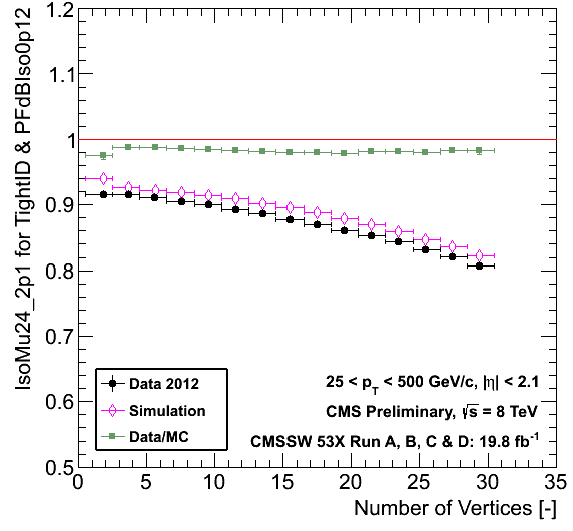
\includegraphics[width=0.3\textwidth,]{figures/trigger/muonEffvsNvtx}
    }   
  \subfigure{
   \includegraphics[width=0.42\textwidth,page=65]{figures/data-mc/v21/mu/muonLook_pfJet_ge2j_375.pdf}
   }\\     
    \caption{\label{fig:eff-muon}
    (left) Muon trigger efficiency as a function of
    number of primary vertices for muon $\pt>$ 25 \gev and
    $|\eta| <$ 2.1. (right) Number of primary vertices
    in muon control sample.} 
 
  \end{center}
\end{figure}

Events for the photon control sample are recorded with the
\verb!HLT_Photon150! trigger, which is $\sim100\%$ efficient for
$E_{\rm T}^{\rm photon} > 165\gev$ and $\scalht > 375\gev$, as shown
in Figure~\ref{fig:eff-photon}. The efficiency measurement is made
using the \verb!HLT_Photon90! trigger as a reference.

\begin{figure}[!h]
  \begin{center}
  \subfigure[\njetlow]{
    \includegraphics[width=0.43\textwidth,page=6]{figures/trigger/g_barrel_375_caloJet_le3j_}
    }   
  \subfigure[\njethigh]{
   \includegraphics[width=0.43\textwidth,page=6]{figures/trigger/g_barrel_375_caloJet_ge4j_}
   }\\     
    \caption{\label{fig:eff-photon}
    Cumulative efficiency turn-on curves for the \texttt{HLT\_Photon150} trigger 
    as a function of photon \pt for events satisfying \njetlow 
    (left) and \njethigh (right).} 
  \end{center}
\end{figure}

\FloatBarrier
